% this file is called up by thesis.tex
% content in this file will be fed into the main document

\chapter{Graphic User Interface Design} % top level followed by section, subsection

\section{Overview}
In chapter 2, I mainly describe the GUI design of the HCMP Player, focus will 
be on how GUI design meet the requirement of HCMP Player, and each GUI components' 
usage and function. Basicly, the GUI of HCMP Player contains 5 components, 
a detailed explaination of each component will be given in following sections. 
Figure 2.1 is a screenshot of GUI of HCMP Player. 

\begin{figure}[H]
\center{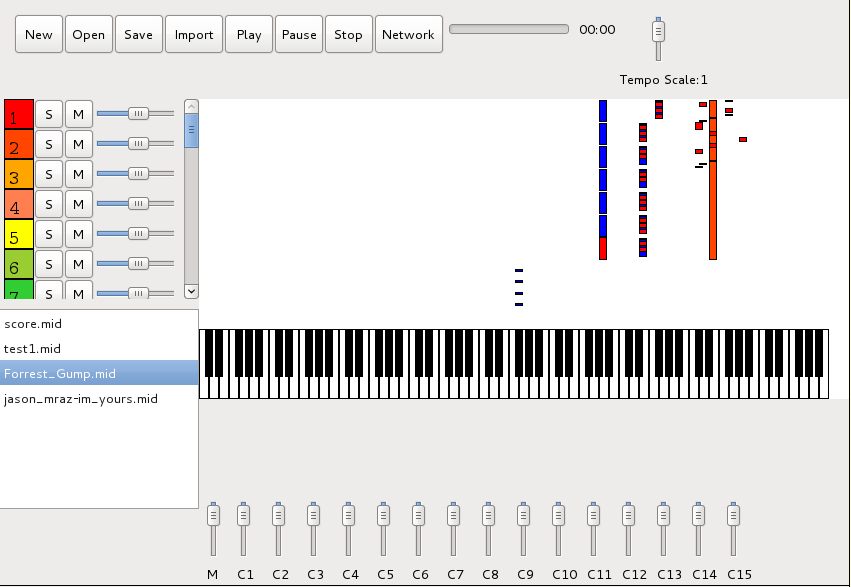
\includegraphics[width=0.75\linewidth]{2/1.png}}
\caption{HCMP GUI Screenshot}
\label{fig:speciation}
\end{figure}

\section{Layout}
Figure 3 is layout of the GUI of HCMP Player. The whole area 
cover 800 * 600 pixels. The top part is the menu panel with 800 * 200 in size. 
Track panel and 
library panel share the middle-left part, ecah is 200 * 200 in size. 
The middle-right part is 400 * 600 in size, which covers the most part of GUI, will be   
a midi keyboard and data display component. The bottom part is the channel   
panel. The bound every component to its own area, I put a container panel at most 
outside layer. The container panel define the boundary GUI of HCMP Player. Any 
component out of this boundary is invible to users. 

\begin{figure}[H]
\center{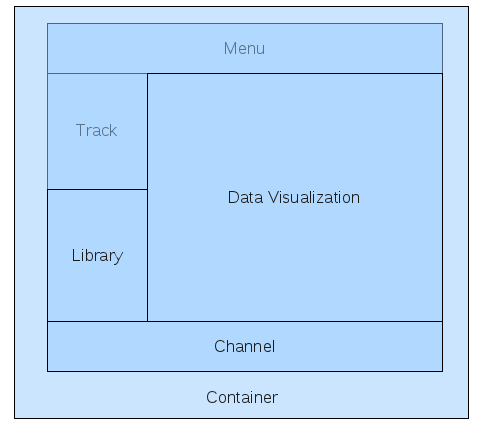
\includegraphics[width=0.6\linewidth]{2/5.png}}
\caption{HCMP Player Layout}
\label{fig:speciation}
\end{figure}

\section{GUI Component}

\subsection{Menu Panel}

Figure 2.3 is the screenshot of menu panel. The menu panel integrate most of control 
functions for HCMP Player. New, open, save buttons form a group, the group is used to 
manipulate configuration file. Play, pause, stop buttons form another group, 
the group is used to directly control the HCMP Player. 
The function of each button just like its name suggest. The network button 
is for HCMP Player  
network function, after clicking the button, the player will try to automatically 
initiate a connection to a remote server, the IP address and port number pair is 
predefined in configuration file and can be easily changed. Once connection is 
successfully built, all the control will then be transferred to the remote server. 
This function will be explained in more detail in following
chapters. Apart from those buttons, menu panel also contain a slider to change 
tempo, the slider inidicate the scale coefficient of tempo value.For example, if the original tempo is 90 BMP, with slider set to scale coefficient 1.5, the tempo will be 1.5 * 90 
BMP when playing the file. The import button is used to import a midi file 
into the HCMP Player, once a midi file is successuflly imported into the HCMP Player  
, track panel, library panel and data display component will all be updated. 
The path of track will also be recorded into the configuration file, so that the user 
will not bother to import the same file again.

\begin{figure}[H]
\center{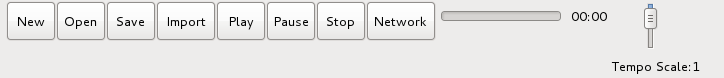
\includegraphics[width=0.8\linewidth]{2/6.png}}
\caption{HCMP Player Menu Panel}
\label{fig:speciation}
\end{figure}

\subsection{Track Panel}

Figure 2.4 is the screenshot of track panel. The track panel is used to 
control each track's parameter, these parameters are volume, solo, mute. Color
block at the front of panel indicate its color in data display component . The 
track panel will automatically be populated once a midi file is successfully 
loaded into HCMP Player. 
\begin{figure}[H]
\center{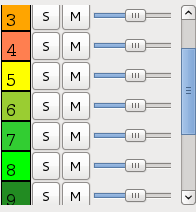
\includegraphics[width=0.3\linewidth]{2/7.png}}
\caption{HCMP Player Track Panel}
\label{fig:speciation}
\end{figure}

\subsection{Midi Keyboard and Data Display}
Figure 2.5 is the screenshot of data display component. It is made up of a virtual  
keyboard and a midi note canvas. After successfuly loading a midi file, the midi 
note canvas will 
draw each midi note to this area. When playing a midi file, midi canvas will 
automatically update the position of each midi note. 

The virtual keyboard has 9 octaves and 108 keys. Both the white key and black key 
are drawn by canvas. Every midi note will be highlighted in the 
virtual midi keyboard based on its pitch while playing. To avoid asynchronized speed 
of canvas update and playing midi note problem. The canvas update speed is 
coordinited with the player engine. Player engine is responsible for beat update and it 
periodically send synchronization information to GUI. After receiving update 
information from player engine, the GUI will update all the midi note in canvas.

Each color of midi note represent a track inside 
a midi file, in current version, color for each track's midi note is predefined. 
Midi canvas scroll speed is linear to the tempo of midi. Whenever user 
make a change to the tempo, the scroll speed of midi canvas will also be adjusted 
accordingly. When a user mute certain 
track, its color midi note in midi canvas will temporarily be set to invisble. 
The canvas
update frequency is about 20Hz. To make logic easier, everytime update event 
happened, the whole midi canvas will be redrawed. The midi canvas is about 400 * 600 
in size, and these pixels are update 20 times every second, which is approximately 
20 frames per second. The performance is not
a major concern. There is canvas buffer data 
structure to store all the ``visble'' midi notes. 
Usually, the size of a midi file is no more than 10MB, the overall performance of 
using redraw method is acceptable.

\begin{figure}[H]
\center{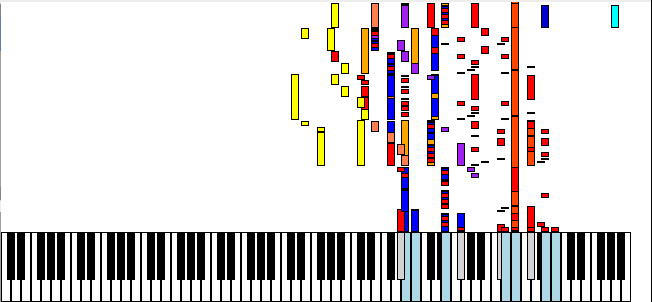
\includegraphics[width=0.7\linewidth]{2/3.png}}
\caption{HCMP Player Data Display Component}
\label{fig:speciation}
\end{figure}

\subsection{HCMP Midi Player Library}

Figure 2.6 is the screenshot of midi library panel. This simple midi library is 
used to remember all the midi file that has ever been successfully loaded . 
A configration file of HCMP Player store all the file name as well as its path, 
so that next time when user launch HCMP Player again, it is able to load these 
recently openned midi files immediately. Everytime a user click any file in the libary, 
The GUI looks up a hash-like data structure and fetch its file path (if exist),
it then is automatically
loaded into the HCMP Player. If the midi file failed to load, the library and its
configuration file will remove the obsolete entry and then update the library panel
agian.

\begin{figure}[H]
\center{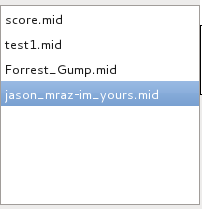
\includegraphics[width=0.3\linewidth]{2/8.png}}
\caption{HCMP Player Library Panel}
\label{fig:speciation}
\end{figure}

\section{Player Mode}

The HCMP Player has two mode, stand-alone mode and network mode. 
In stand-alone mode, HCMP Player can be used as normal midi player 
, user could load and play midi file. In network mode, 
the HCMP Player will connect to a remote 
server, in HCMP project, the server usually contains a conductor, and this
conductor is responsible for communication and coordination with all the 
instance of HCMP Players. For example, 
a typical workflow of conductor is to read cue from external resource, 
then issue command all the connected instances of the HCMP Players.

\subsection{Stand-alone Mode}

When lauching the program, the HCMP player is default in stand-alone mode, 
all the GUI component's function is described like above. 
User could use HCMP Player to play midi file, change tempo, change volume, etc.


\subsection{Network Mode}

After launching the HCMP Player, if user click the network button, 
the HCMP player will try to enter into    
the network mode. At the beginning, it initiate a connection request 
to remote server, the address and port number will stored in the
HCMP Player configuration file. If receving no reply within certain 
timeout period, the HCMP player ``rollback'' to its stand-alone mode.
If receving confirm signal from
remote server, the 2-way connection between the HCMP Player and 
remote server is successfully built up. Then, the HCMP Player and 
remote server is able to communicate with each other. The control of HCMP 
Player will partially be ``transfered'' to remote server. 
In this mode, player control buttons like play, pause   
, stop still work as normal, to avoid conflict problems, other buttons will 
be temporarily disabled, which means binding method for these buttons is replaced by
another set of functions. The detailed network API information will be explained  
in the chapter 5.
